\documentclass{beamer}

\mode<presentation> {

%\usetheme{default}
%\usetheme{AnnArbor}
%\usetheme{Antibes}
%\usetheme{Bergen}
%\usetheme{Berkeley}
%\usetheme{Berlin}
%\usetheme{Boadilla}
%\usetheme{CambridgeUS}
%\usetheme{Copenhagen}
%\usetheme{Darmstadt}
%\usetheme{Dresden}
%\usetheme{Frankfurt}
%\usetheme{Goettingen}
%\usetheme{Hannover}
%\usetheme{Ilmenau}
%\usetheme{JuanLesPins}
%\usetheme{Luebeck}
\usetheme{Madrid}
%\usetheme{Malmoe}
%\usetheme{Marburg}
%\usetheme{Montpellier}
%\usetheme{PaloAlto}
%\usetheme{Pittsburgh}
%\usetheme{Rochester}
%\usetheme{Singapore}
%\usetheme{Szeged}
%\usetheme{Warsaw}


%\usecolortheme{albatross}
%\usecolortheme{beaver}
%\usecolortheme{beetle}
%\usecolortheme{crane}
%\usecolortheme{dolphin}
%\usecolortheme{dove}
%\usecolortheme{fly}
%\usecolortheme{lily}
%\usecolortheme{orchid}
%\usecolortheme{rose}
%\usecolortheme{seagull}
%\usecolortheme{seahorse}
%\usecolortheme{whale}
%\usecolortheme{wolverine}

%\setbeamertemplate{footline} % To remove the footer line in all slides uncomment this line
%\setbeamertemplate{footline}[page number] % To replace the footer line in all slides with a simple slide count uncomment this line

%\setbeamertemplate{navigation symbols}{} % To remove the navigation symbols from the bottom of all slides uncomment this line
}

\usepackage{graphicx} % Allows including images
\usepackage{booktabs} % Allows the use of \toprule, \midrule and \bottomrule in tables
\usepackage{amsfonts}
\usepackage{mathrsfs, bbold}
\usepackage{amsmath,amssymb,graphicx}
\usepackage{mathtools} % gather
\usepackage[export]{adjustbox} % right-aligned graphics

%----------------------------------------------------------------------------------------
%	TITLE PAGE
%----------------------------------------------------------------------------------------

\title["11"]{11: Basics of Markov chain Monte Carlo Simulation}

\author{Taylor} 
\institute[UVA] 
{
University of Virginia \\
\medskip
\textit{} 
}
\date{} 

\begin{document}
%----------------------------------------------------------------------------------------

\begin{frame}
\titlepage 
\end{frame}

%----------------------------------------------------------------------------------------
\begin{frame}
\frametitle{Introduction}

In this section, we discuss {\bf Markov chain Monte Carlo} techniques, which all produce \underline{correlated} draws from the posterior of interest.


\end{frame}

%----------------------------------------------------------------------------------------
\begin{frame}
\frametitle{Overview}

Even though we might not even have a time series model, we construct a Markov chain 
$$
\theta^1, \theta^2, \ldots, \theta^N
$$
Even though these draws are correlated, they are all {\bf marginally} distributed according to the posterior 
$$
p(\theta \mid y).
$$
We estimate expectations with sample means:
$$
E[h(\theta) \mid y] \approx  \frac{1}{N}\sum_{i=1}^N h(\theta^i).
$$
\end{frame}

%----------------------------------------------------------------------------------------
\begin{frame}
\frametitle{Typical MCMC Output}

A 2-parameter model:
\begin{center}
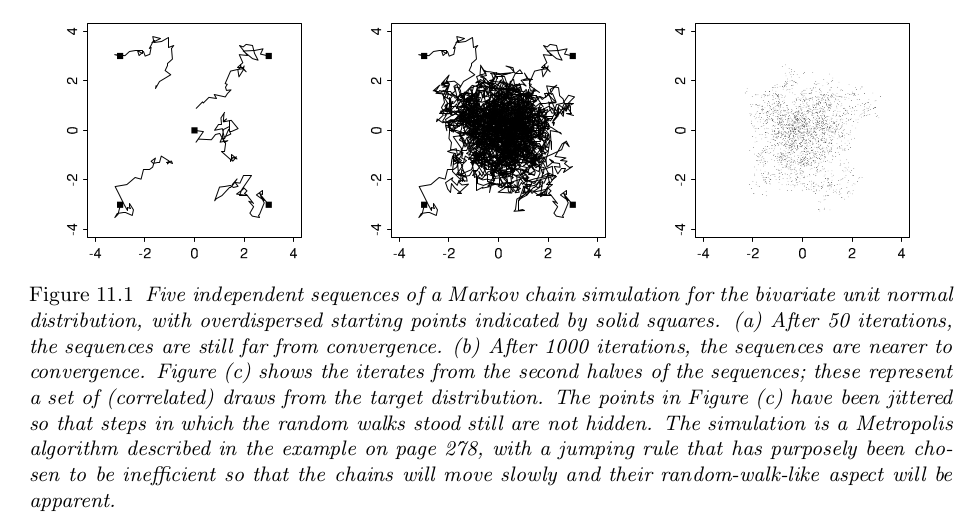
\includegraphics[width=120mm]{fig11.png}
\end{center}

\end{frame}




%----------------------------------------------------------------------------------------
\begin{frame}
\frametitle{Typical MCMC Output}

Another 2-parameter model:

\begin{center}
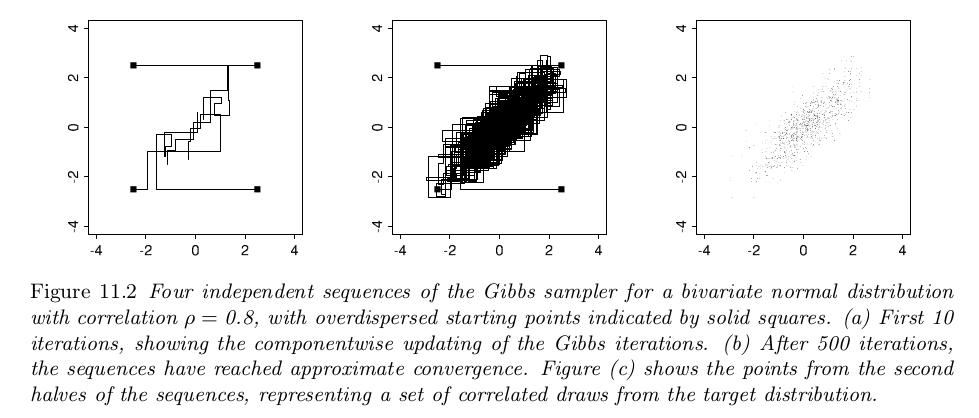
\includegraphics[width=120mm]{gibbs.png}
\end{center}

\end{frame}




%----------------------------------------------------------------------------------------
\begin{frame}
\frametitle{Typical MCMC Output}

A 6-parameter model from: \url{https://academic.oup.com/jfec/article/14/2/278/1751519}

\begin{center}
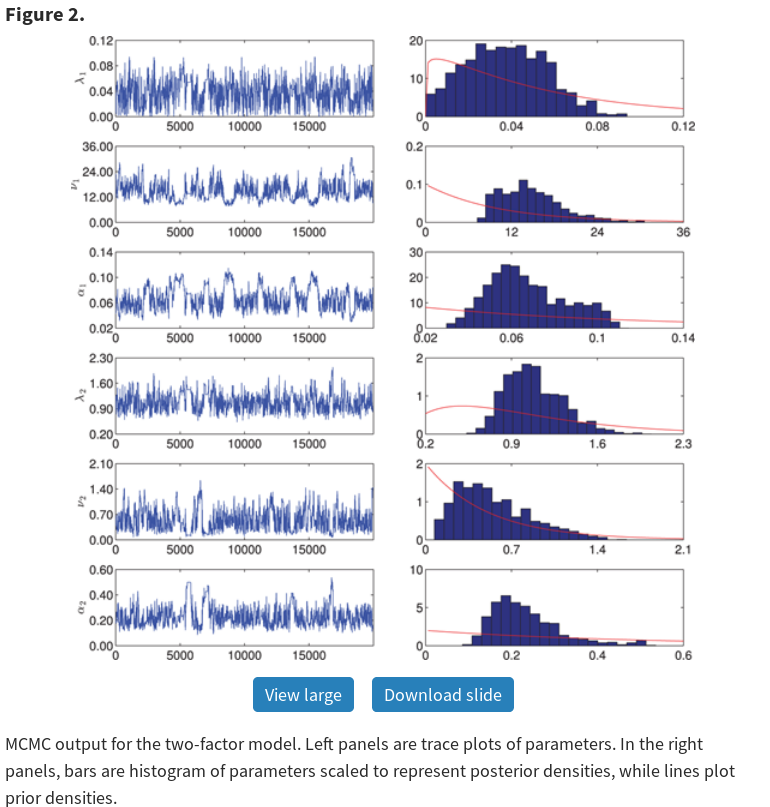
\includegraphics[width=70mm]{trace_hist.png}
\end{center}

\end{frame}

%----------------------------------------------------------------------------------------
\begin{frame}
\frametitle{Variance of our Estimator}

Let $\sigma^2 = \operatorname{Var}[h(\theta^i)]$, $\rho(h) = \operatorname{Corr}\left(  h(\theta^i), h(\theta^{h+i}) \right)$
\begin{align*}
N \operatorname{Var}\left[ \frac{1}{N}\sum_{i=1}^N h(\theta^i) \right] &= N\operatorname{Cov}\left( \frac{1}{N}\sum_{i=1}^N h(\theta^i),\frac{1}{N}\sum_{j=1}^N h(\theta^j) \right) \\
&= \frac{1}{N} \sum_{i=1}^N\sum_{j=1}^N\operatorname{Cov}\left(  h(\theta^i), h(\theta^i) \right) \tag{bilinearity} \\
&= \sigma^2 \left\{ 1 + 2\sum_{h=1}^N \frac{N - h}{N} \rho(h)\right\}  \tag{count diagonally} \\
&\to \sigma^2 \underbrace{\left\{ 1 + 2\sum_{h=1}^{\infty}  \rho(h)\right\}}_{\text{correlation is bad}} 
\end{align*}



\end{frame}


%----------------------------------------------------------------------------------------
\begin{frame}
\frametitle{Typical MCMC Output}

Assessing the integrated autocorrelation with acf plots:
\begin{center}
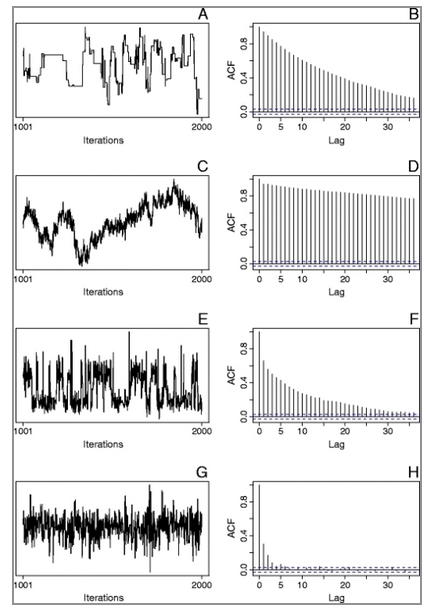
\includegraphics[width=40mm]{autocorr.png}
\end{center}
bad, bad, less bad, good.
\url{https://openi.nlm.nih.gov/detailedresult?img=PMC3218285_13428_2011_114_Fig10_HTML&req=4}

\end{frame}

%----------------------------------------------------------------------------------------
\begin{frame}
\frametitle{Another issue}

The previous problem assumes each draw is distributed according to the posterior. 
\newline

If we start the chain far away from the mode, how long until it converges? How can we be sure it has converged?
\newline
\pause

Trace plots help. We also have convergence diagnostics (more on this later).
\newline

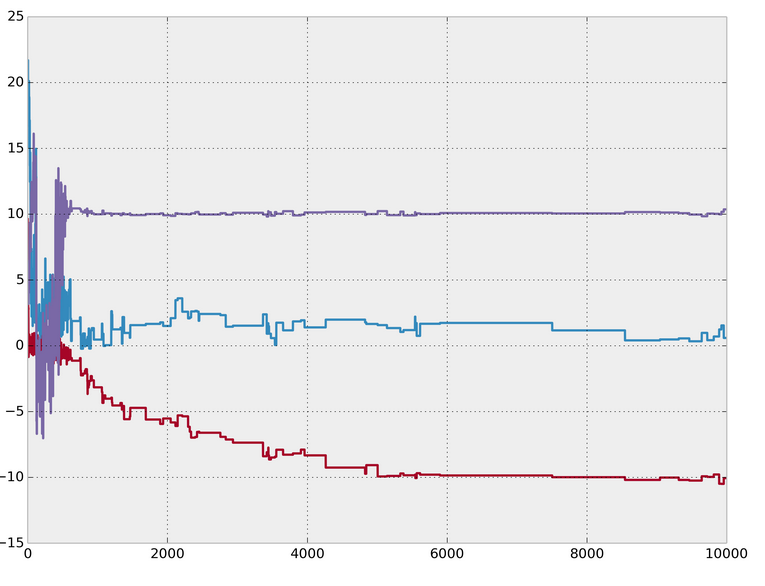
\includegraphics[width=40mm]{convergence.png} You could throw away $6000$ iterations as a {\bf burn in} or {\bf warm-up}.

\end{frame}


%----------------------------------------------------------------------------------------
\begin{frame}
\frametitle{Metropolis-Hastings algorithm}

At iteration $t-1$ you have $\theta^{t-1}$. Propose $\theta^* \sim q(\theta \mid \theta^{t-1})$, and accept this draw with probability 
$$
a(\theta^{t-1}, \theta^*) = \min\left\{1, \frac{p(\theta^* \mid y)q(\theta^{t-1} \mid \theta^*) }{p(\theta^{t-1} \mid y) q(\theta^* \mid \theta^{t-1}) }\right\}.
$$
If you accept, $\theta^t = \theta^*$. Otherwise, $\theta^t = \theta^{t-1}$. 
\newline

{\it Many} algorithms are a special case of this one.

\end{frame}
%----------------------------------------------------------------------------------------
\begin{frame}
\frametitle{Metropolis-Hastings algorithm}

Why it's widely-applicable:
\begin{align*}
a(\theta^{t-1}, \theta^*) &= \min\left\{1, \frac{p(\theta^* \mid y)q(\theta^{t-1} \mid \theta^*) }{p(\theta^{t-1} \mid y) q(\theta^* \mid \theta^{t-1}) }\right\} \\
&= \min\left\{1, \frac{p(\theta^*, y)/p(y)q(\theta^{t-1} \mid \theta^*) }{p(\theta^{t-1}, y)/p(y) q(\theta^* \mid \theta^{t-1}) }\right\} \\
&= \min\left\{1, \frac{p(y \mid \theta^*) p(\theta^*)q(\theta^{t-1} \mid \theta^*) }{p(y \mid \theta^{t-1}) p(\theta^{t-1}) q(\theta^* \mid \theta^{t-1}) }\right\}.
\end{align*}
Don't need to know the normalizing constant/marginal likelihood/evidence!

\end{frame}
%----------------------------------------------------------------------------------------
\begin{frame}
\frametitle{Metropolis-Hastings algorithm}

$$
a(\theta^{t-1}, \theta^*) = \min\left\{1, \frac{p(\theta^* \mid y)q(\theta^{t-1} \mid \theta^*) }{p(\theta^{t-1} \mid y) q(\theta^* \mid \theta^{t-1}) }\right\}.
$$

\begin{enumerate}
\item When is $a(\theta^{t-1}, \theta^*)$ big?
\item When is $a(\theta^{t-1}, \theta^*)$ small?
\item How should we pick $q(\theta^* \mid \theta^{t-1})$?
\item What is the ideal $q(\theta^* \mid \theta^{t-1})$?
\item What if $q(\theta^* \mid \theta^{t-1})$ is too peaked?
\item What if $q(\theta^* \mid \theta^{t-1})$ is too diffuse?
\end{enumerate}


\end{frame}
%----------------------------------------------------------------------------------------
\begin{frame}
\frametitle{Metropolis-Hastings algorithm}

Let's pick $q(\theta \mid \theta^{t-1}) = \text{Normal}(\theta^{t-1}, \sigma^2 {\bf I} )$
\newline

\url{https://chi-feng.github.io/mcmc-demo/app.html\#RandomWalkMH,banana}
\end{frame}



%----------------------------------------------------------------------------------------
\begin{frame}
\frametitle{Independent Metropolis Hastings}

If $q(\theta \mid \theta^{t-1}) = q(\theta)$ (i.e. propose independently of past values), then you have the {\bf Independent Metropolis Hastings} algorithm, which has acceptance probabilities
$$
a(\theta^{t-1}, \theta^*) = \min\left\{1, \frac{p(\theta^* \mid y)q(\theta^{t-1} ) }{p(\theta^{t-1} \mid y) q(\theta^* ) } \right\}.
$$

The proposals are iid, but the chain is Markovian!

\end{frame}

%----------------------------------------------------------------------------------------
\begin{frame}
\frametitle{Metropolis algorithm}

If $q(\theta^* \mid \theta^{t-1}) = q(\theta^{t-1} \mid \theta^*)$ (i.e. $q$ is {\bf symmetric}), the acceptance probability
$$
a(\theta^{t-1}, \theta^*) = \min\left\{1, \frac{p(\theta^* \mid y)q(\theta^{t-1} \mid \theta^*) }{p(\theta^{t-1} \mid y) q(\theta^* \mid \theta^{t-1}) }\right\}.
$$
becomes
$$
a(\theta^{t-1}, \theta^*) = \min\left\{1, \frac{p(\theta^* \mid y)}{p(\theta^{t-1} \mid y)  }\right\}.
$$
and they call this the {\bf Metropolis} algorithm (drop the ``Hastings").

\end{frame}

%----------------------------------------------------------------------------------------
\begin{frame}
\frametitle{The Gibbs Sampler}

Say there are two parameters: $\theta = (\theta_1, \theta_2)$. The {\bf Gibbs sampler} alternates between 
\begin{enumerate}
\item $\theta_1^t \sim p(\theta_1 \mid \theta_2^{t-1}, y)$
\item $\theta_2^t \sim p(\theta_2 \mid \theta_1^{t}, y)$
\end{enumerate}

If there are more parameters: $\theta = (\theta_1, \theta_2, \ldots, \theta_d)$. The Gibbs sampler alternates between 
\begin{enumerate}
\item $\theta_1^t \sim p(\theta_1 \mid \theta_{2:d}^{t-1}, y)$
\item $\theta_2^t \sim p(\theta_2 \mid \theta_1^t, \theta_{3:d}^{t-1}, y)$
\item $\vdots$
\item $\theta_d^t \sim p(\theta_d \mid \theta_{1:d-1}^{t}, y)$
\end{enumerate}

This is only possible if you can sample from the {\bf conditional posteriors} (i.e. need conditional conjugacy).

\end{frame}

%----------------------------------------------------------------------------------------
\begin{frame}
\frametitle{The Gibbs Sampler}

Example on page 277:
\begin{enumerate}
\item $\theta_1 \mid \theta_2, y \sim \text{Normal}(y_1 + \rho(\theta_2 - y_2), 1-\rho^2)$
\item $\theta_2 \mid \theta_1, y \sim \text{Normal}(y_2 + \rho(\theta_1 - y_1), 1-\rho^2)$
\end{enumerate}

\begin{center}
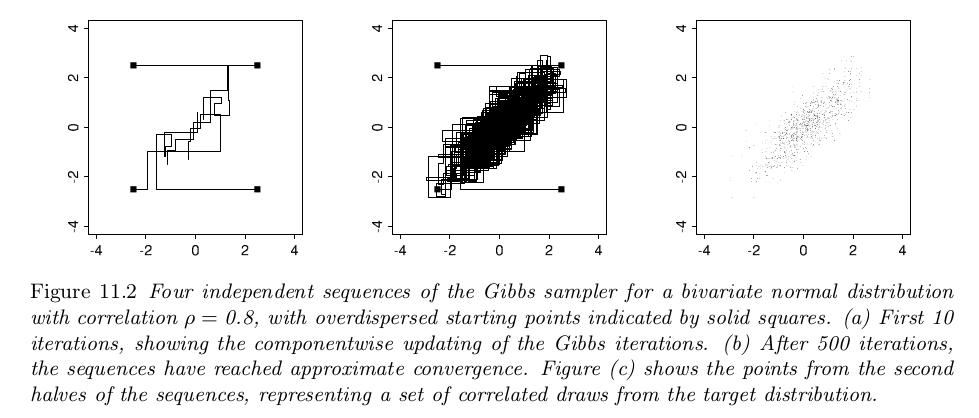
\includegraphics[width=80mm]{gibbs.png}
\end{center}


\end{frame}

%----------------------------------------------------------------------------------------
\begin{frame}
\frametitle{Back to  Assessing convergence for scalars $\psi_{i,j}$}

Run $m$ chains for $n$ iterations, $i=1,\ldots,n$ and $j=1\ldots,m$.
\begin{align*}
\bar{\psi}_{\cdot \cdot} &= \frac{1}{mn}\sum_{i=1}^n\sum_{j=1}^m \psi_{ij} \tag{overall average} \\
\bar{\psi}_{\cdot j} &= \frac{1}{n}\sum_{i=1}^n \psi_{ij} \tag{chain average} \\
s^2_j &= \frac{1}{n-1}\sum_{i=1}^n (\psi_{ij}-\bar{\psi}_{\cdot j})^2 \tag{chain sd} \\
W &= \frac{1}{m} s^2_j \tag{within-sequence variance} \\
B &= \frac{n}{m-1} \sum_{j=1}^m (\bar{\psi}_{\cdot j} - \bar{\psi}_{\cdot \cdot})^2\\
\hat{\text{var}}^{+}(\psi \mid y) &=\frac{n-1}{n}W + \frac{1}{n}B.
\end{align*}



\end{frame}
\end{document} 
